\chapter{Модель Mb-Lock} \label{chapt2}

\section{Требования к разрабатываемой модели} \label{sect2_1}

Проектирование и разработка модели проводилось исходя из следующих требований,
вытекающих из практических свойст СКУД и недостатков существующих решений:
\begin{enumerate}
	\item Реализации идеи использования смартфона в качестве ключа.
	\item Поддержка биометрической верификации пользователя.
	\item Простота системы для конечных пользователей, сравнимая с обычными механических ключами и смарт-картами.
	\item Производительность системы для конечных пользователей, сравнимая с обычными механических ключами и смарт-картами.
	\item Единая точка для администрирования системы.
	\item Отсутствие необходимости подключения устройства замка к внешней локально-вычислительной сети.
	\item Базовая поддержка многопользовательского режима.
	\item Возможность удаленного контроля доступом (предоставление доступа, отмена доступа, политики доступа).
	\item Возможность предоставления доступа на определенный период времени.
	\item Безопасность системы как в случае внешних так и в случае внутренних атак.
	\item Поддержка технологий NFC, Bluetooth, WiFi, WiFi Direct для коммуникации между мобильным устройством пользователя и контроллером замка.
	\item Простота внедрения системы (отсутствие необходимости глобальных изменений в существующей инфраструктуре помещения при внедрении, отсутствие необходимости подключения контроллера замка к локальной или глобальной вычислительной сети).
	\item Отказоустойчивость и модель аварийного доступа.
	\item Возможность использования сопряжения с существующими электро-механическими замки.
\end{enumerate}

\section{Архитектура системы} \label{sect2_2}

В рамках сформулированных требований сложной исследовательской задачей стала разработка архитектуры системы и алгоритмов взаимодействия ее различных элементов, с учетом обеспечения целостной безопасности и удобство использования. 

\begin{figure}[ht] %
\centering
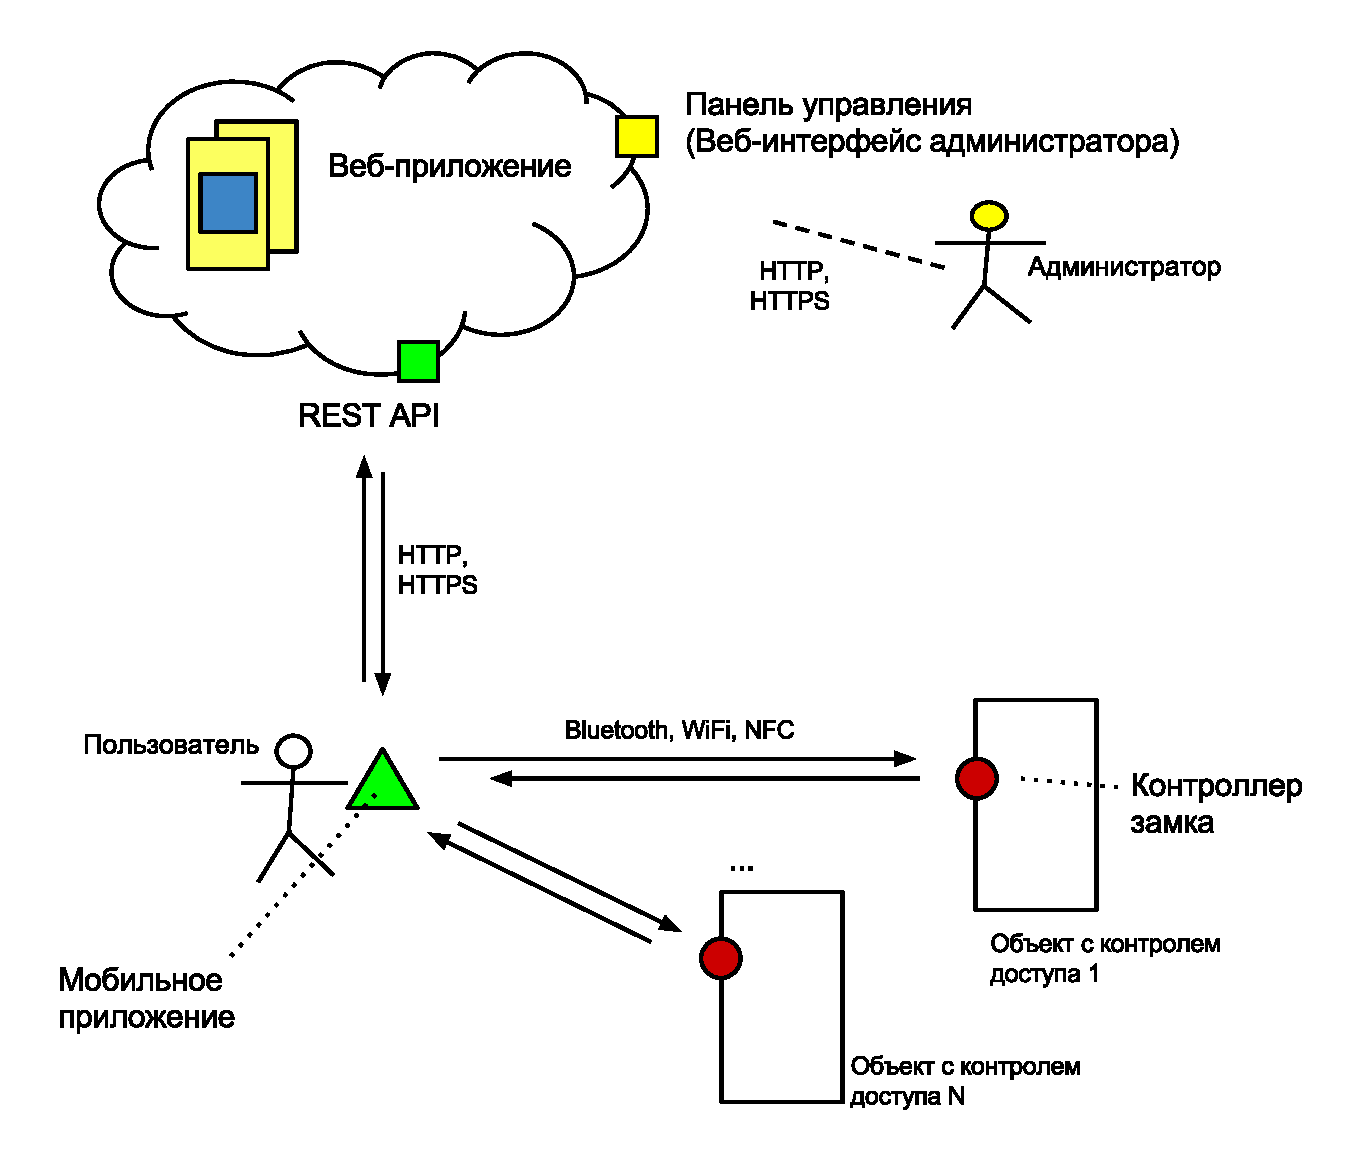
\includegraphics[scale=0.4]{mblock_arch}\\
% Указывается размер рисунка (каким Вы его хотите видеть)% и имя вставляемого файла
\caption{Архитектура системы}% Подпись рисунка должна быть обязательно
\label{mblock_arch}% Метка для ссылки на рисунок.
\end{figure}

С точки зрения архитектуры разработанная архитектура системы содержит три основных взаимодействующих между собой компонента — \textbf{мобильное приложение} на устройстве пользователя, 	приложение контроллера замка} и \textbf{веб-приложение}. 

Мобильное приложение устанавливается на каждое устройство каждого пользователя, после процедуры активации устройство может использоваться в качестве ключа для всех объектов для которых у пользователя разрешен доступ.

Приложение контроллера замка устанавливается на микроконтроллер замка, который можем быть встроен замок или являться отдельным логическим элементом, сопрягаемым с замком. Ключевой особенностью разработанной модели является отсутствие необходимости взаимодействия между контроллером замка и веб-приложением в режиме эксплуатации системы. 

Веб-приложение имеет единственную копию в рамках всей системы и состоит из двух взаимосвязанных компонентов:
\begin{enumerate}
	\item \textbf{Панель управления (веб-интерфейс администратора)} является браузерным приложением и предназначена для удаленного управления системой администраторами. Доступ к панели управления имеют только администраторы системы, при этом физическая безопасность гарантируется самим предприятием или облачным сервисом, который используется для разворачивания приложения.

	\item \textbf{REST API} является эталонной реализацией подхода REST, работает в автоматическом режиме и служит для взаимодействия между мобильным приложением и веб-приложением, на основе настроек сделанных в панели управления.
\end{enumerate}

Стоит отметить, что в случае использовании системы в массовом / персональном сегменте веб-приложение может быть развернуто в виде SaaS сервиса, работающего в режиме 24/7, что не требует от обычных пользователей никаких дополнительных действий по разворачиванию и поддержке веб-приложения. С другой стороны, большие предприятия могут размещать веб-приложение на собственных локально-вычислительных ресурсах, что гарантирует им безопасность и полный контроль доступа к веб-приложению. В любом случае веб-приложение является единой и защищенной точкой для администрирования всей системой.

\section{Пользовательские сценарии} \label{sect2_3}

Разработанная модель системы предполагает пользовательские сценарии описанные в данном разделе. При этом стоит отметить что с практической точки зрения в зависимости от области применения сценарии могут различаться. 

\begin{itemize}
	\item В случае персональной системы доступа, владелец замка является одновременно администратором системы и ее пользователем, и в большинстве случаев не нуждается в настройке сложных политик доступа и биометрических проверках. 

	\item В случае промышленного использования на предприятиях, владелец предприятия а также уполномоченные сотрудники предприятия могут выступать в роли администраторов системы. Остальные сотрудники предприятия выступают в качестве пользователей системы и не имеют доступа к панели управления. Также для данного случая крайне важна точная настройка политик доступа и возможность использовании биометрической верификации для ключевых объектов предприятия.
\end{itemize} 

В рамках данной работы пользовательские сценарии будут рассмотрены для случая многопользовательской системы доступа предприятия имеющего высокие требования к безопасности. Стоит отметить, что данный вариант является наиболее сложным и объемным, в том смысле, что большинство других вариантов могут получены из данного путем исключения избыточных сценариев.

\subsection{Сценарий 1. Закупка} \label{subsect2_3_1}

Предприятие закупает оборудование (замки со встроенным контроллером или только только контроллеры замков при использовании электро-механических замков на предприятии) и получает доступ к панели управления. В веб-приложении сохраняются email-ы и номера телефонов сотрудников, ответственных за непрерывную работоспособность системы (администраторов системы).

\subsection{Сценарий 2. Установка и активация} \label{subsect2_3_2}

Администраторы совместно с техническими специалистами предприятия производят установку замков и активацию каждого контроллера замка. Активация осуществляется с помощью специального \textbf{мобильного приложения администратора}. Также на каждом контроллере замка необходимо установить точное время.

После активации контроллера замка, замок появляется в инфраструктуре предприятия в панели управления. Для каждого замка можно указать легкое и понятное имя замка (например, кабинет 212, серверная, конференц-зал и т.п.).

Питание контроллера происходит от внутреннего аккумулятора, емкость которого может быть выбрана в зависимости от условий эксплуатации, при этом аккумулятор является подзаряжаемым, в том числе возможна постоянная подзарядка от внешней электрической сети, или периодическая плановая подзарядка по штатному техническому расписанию предприятия. При обнаружении малого уровня заряда аккумулятора администраторы системы получают уведомление, в котором содержится введенное ранее название замка и последние известный уровень заряда.

Также стоит отметить, что при бездействии или халатности со стороны администраторов и критически малом уровне заряда, контроллер замка переводит замок в открытое состояние.

\subsection{Сценарий 3. Настройка политики доступа} \label{subsect2_3_3}

В панели управления отображается текущая инфраструктура здания и все активированные замки, включая информацию об их текущем состоянии. Также в панели управления отображается текущий список сотрудников компании. Администраторы имеют возможность \textbf{настройки политики доступа} — редактирования списка сотрудника и настройки прав доступ для каждого сотрудника в отдельности

При добавлении нового сотрудника указывается его Имя Фамилия, email, номер телефона, и любая другая необходимая мета-информация. После формирования списка сотрудников, администраторы имеют возможность при помощи настройки политики доступа контролировать права доступа каждого сотрудника относительно всех объектов предприятия оснащенных контроллерами.

Еще одним базовым изменяемым параметром системы является \textbf{время жизни токена пользователя (User Token Life Time, UTLT)}. 

По-умолчанию UTLT = 24 часа. Практически это означает, что администратор не может забрать доступ у сотрудника быстрее чем за 24 часа. С другой стороны для сотрудника время UTLT является максимально возможным временем в течении которого мобильное приложение сотрудника может не иметь доступа в интернет без потери доступа к объектам системы. Администраторы имеют возможность контроля значения параметра UTLT.

\subsection{Сценарий 4. Процедура активации устройства} \label{subsect2_3_4}

При первом получении права доступа со стороны администраторов сотрудник получает  электронное письмо, содержащее уникальную секретную ссылку. 

При открытии секретной ссылки с мобильного устройства запускается мобильное приложение, которое устанавливает связь с веб-приложение и безопасным образом активирует доступ пользователя. После этого мобильное устройства сотрудника на котором была произведена активация превращается в персональный ключ для всех разрешенных согласно политики доступа объектов. 

\begin{figure}[ht] %
	\centering
	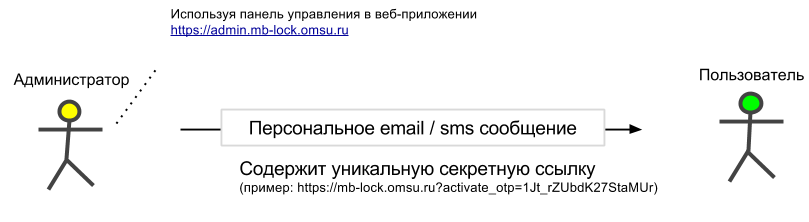
\includegraphics[scale=0.4]{mblock_otp}\\ % Указывается размер рисунка (каким Вы его хотите видеть)% и имя вставляемого файла
	\caption{Сообщение с секретной ссылкой активации}% Подпись рисунка должна быть обязательно
	\label{mblock_otp}% Метка для ссылки на рисунок.
\end{figure}

Ссылка активации является одноразовой поэтому в случае удаления приложения, потери или замены смартфона, сотрудник должен обратиться к администраторам системы для повторного получения доступа и блокировки старого.

Также стоит отметить, что у сотрудника компании нет необходимости регистрации в системе.

\subsection{Сценарий 5. Взаимодействие с системой со стороны сотрудника} \label{subsect2_3_5}

После прохождения процедуры активации устройства в мобильном приложении отображается список всех разрешенных объектов для сотрудника. При этом для открытия замка достаточно нажать на соответствующей ей элемент списка в мобильном приложении. 
После запроса открытия замка мобильное приложение связывается с контроллером замка.

\begin{itemize}
	\item В случае успеха происходит открытие двери или получение доступа к целевому объекту. 
	\item В случае ошибки пользователю показывается подробная информация о причинах ошибки и возможных путях к ее устранению.
\end{itemize}

\subsection{Сценарий 6. Биометрическая верификация} \label{subsect2_3_6}

В некоторых случаях предприятию необходимо гарантия того, что доступ предоставляется только определенному списку сотрудников, а любой другой человек не имеет возможности получить доступ даже при использовании устройства доверенного сотрудника. В подобных случаях администраторы системы имеют возможность включения биометрическую верификацию для необходимого списка объектов.
 
При включении биометрической верификации, мобильное приложение в момент попытки доступа к биометрически-защищенному объекту генерирует случайную фразу и просит пользователя сказать ее. По-умолчанию, пользователю дается 5 секунд (контролируемый параметр) на то чтобы сказать фразу. 

После захвата ответа пользователя мобильное приложение производит верифицирует голос пользователя и проверяет совпадение сказанной фразы с оригинальным вариантом. 

\begin{itemize}
	\item В случае положительного результата, происходит связь с контроллером замка и его открытие аналогично сценарию 5. 
	\item В случае непрохождения биометрической верификации, пользователю предлагается повторить попытку, при этом каждый раз генерируется новая случайная фраза.
\end{itemize}

\subsection{Сценарий 7. Изменение политики доступа} \label{subsect2_3_7}

При увольнении сотрудника или при изменении его полномочий, администраторы системы имеют возможность изменения настройки политики доступа. 

\begin{itemize}
	\item При этом при следующем установлением соединения между мобильным приложением и Rest API, практические возможности доступа сотрудника будут синхронизированы с обновленными настройками политики доступа.
	\item При отсутствии соединения между мобильном приложением и REST API сотрудник будет иметь возможность доступа согласно старой настройки политики времени доступа в течение времени не превосходящего время UTLT.
\end{itemize}

Таким образом, администраторы системы не имеют возможности гарантированно забрать доступ за время меньшее чем UTLT, но эта особенность не является дефекетом модели с практической точки зрения, и вызвана требованием отсутствия необходимости подключения замка к локально-вычислительной сети.

\section{Алгоритмы}	\label{sect2_4}

В данном разделе подробно описаны алгоритмы взаимодействия и поведения различных компонентов системы.

\subsection{Алгоритмы активации} \label{subsect2_4_1}

При активации замка при помощи мобильного приложения администратора генерируется и передается на сервер передается уникальный и секретный симметричный ключ замка \textbf{Lock\_Key}, который сохраняется в БД веб-приложения. Таким образом ключ замка известен только веб-приложению и самому замку, а также неявно администраторам системы.

\begin{figure}[ht] %
	\centering
	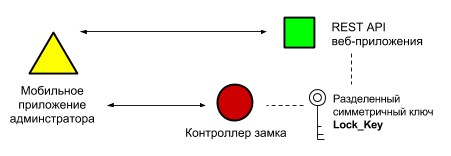
\includegraphics[scale=0.5]{mblock_lock_key}\\ % Указывается размер рисунка (каким Вы его хотите видеть)% и имя вставляемого файла
	\caption{Разделение секретного ключа контроллера замка}% Подпись рисунка должна быть обязательно
	\label{mblock_lock_key}% Метка для ссылки на рисунок.
\end{figure}

При добавлении нового пользователя в систему веб-приложение формирует объект пользователя и генерирует для него уникальный и секретный одноразовый пароль для активации \textbf{Activate\_OTP}, сохраняя соответствие между Activate\_OTP и объектом пользователя в БД. С технической точки зрения Acitvate\_OTP является One Time Password и его генерация должна происходить согласно алгоритмам описанным в RFC.

После получения пользователем письма с уникальной секретной ссылкой и переходом по этой ссылке, запускается мобильное приложение, которое имеет возможность получить значение параметра Activate\_OTP. 

\begin{figure}[ht] %
	\centering
	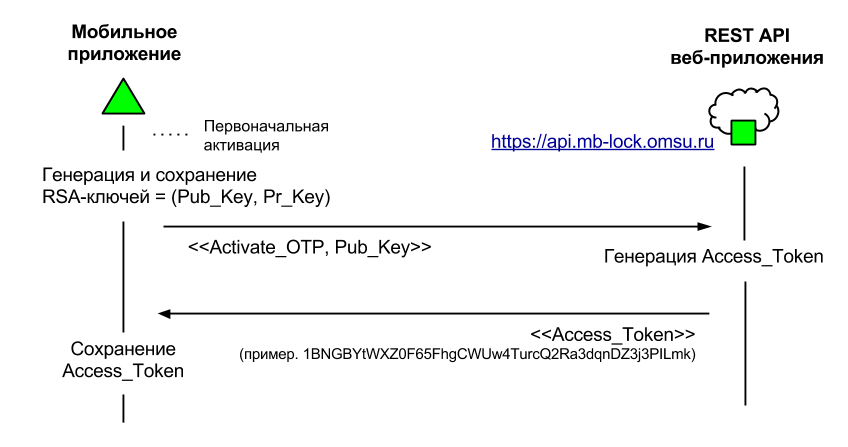
\includegraphics[scale=0.4]{mblock_access_tokens}\\ % Указывается размер рисунка (каким Вы его хотите видеть)% и имя вставляемого файла
	\caption{Активация и получение Access\_Token}% Подпись рисунка должна быть обязательно
	\label{mblock_access_token}% Метка для ссылки на рисунок.
\end{figure}

В момент процедуры активации мобильное приложение генерирует пару открытый-закрытый ключ, которая сохраняется в памяти устройства. 

Веб-приложению сообщается только открытый ключ Pub\_Key, а также Activate\_OTP. В этот момент веб-приложение производит ассоциацию открытого ключа пользователя и ранее созданного пользователя.

Веб-приложение сообщает пользователю Access\_Token, который является псевдо-случайным UUID длины 256 байт.

\subsection{Алгоритм получения Token-ов} \label{subsect2_4_2}

\begin{figure}[ht] %
	\centering
	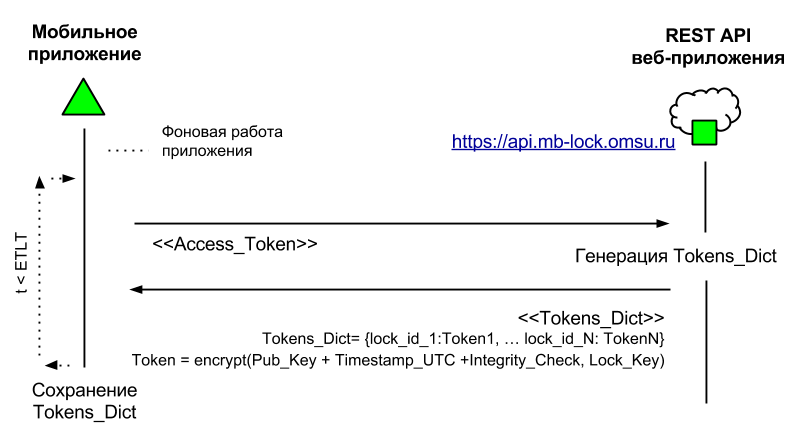
\includegraphics[scale=0.4]{mblock_tokens}\\ % Указывается размер рисунка (каким Вы его хотите видеть)% и имя вставляемого файла
	\caption{Получение токенов}% Подпись рисунка должна быть обязательно
	\label{mblock_tokens}% Метка для ссылки на рисунок.
\end{figure}

Используя Access\_Token мобильное приложение может получать набор токенов Tokens\_Dict. Каждый токен в этом наборе соответствует определенному контроллеру замка, для которого у пользователя есть доступ согласно настройкам в панели управления. При этом токены генерируется по следующему правилу:

\textbf{Token = }encrypt(Pub\_Key + Timestamp\_UTC + Integrity\_Check, Lock\_Key), где

\noindent Pub\_Key — открытый ключ пользователя, Timetamp\_UTC — время в формате UTC до которого валиден Token (по-умолчанию равно текущее время UTC + UTLT), Integrity\_Check — контрольная заранее известная фраза, Lock\_Key – симметричный ключ замка, encrypt — функция симметричного шифрования.

В интерфейсе пользователя мобильного приложения отображаются только те замки, токены для которых известны мобильному приложению. При запросе пользователя на открытие определенного замка мобильное приложение устанавливает соединение с контроллером замка, при этом могут быть использован любой из каналов связи поддерживаемый современными смартфонами: Bluetooth, WiFi, WiFi Direct, NFC.

Стоит отметить, что на данный момент стандарт Bluetooth поддерживается практически всеми современными смартфонами, что является преимуществом разработанной при ее практической реализации и эксплуатации. Также стоит что перехват злоумышленником токена не является проблемой с точки зрения безопасности, что позволяет устанавливать соединение Bluetooth без процедуры Pairing.

Каждый токен является валидным до момента времени Timestamp\_UTC, таким образом мобильному приложению достаточно получить набор токенов один раз за время UTLT (по-умолчанию 24 часа).

\subsection{Алгоритм получения доступа} \label{subsect2_4_3}

\begin{figure}[ht] %
	\centering
	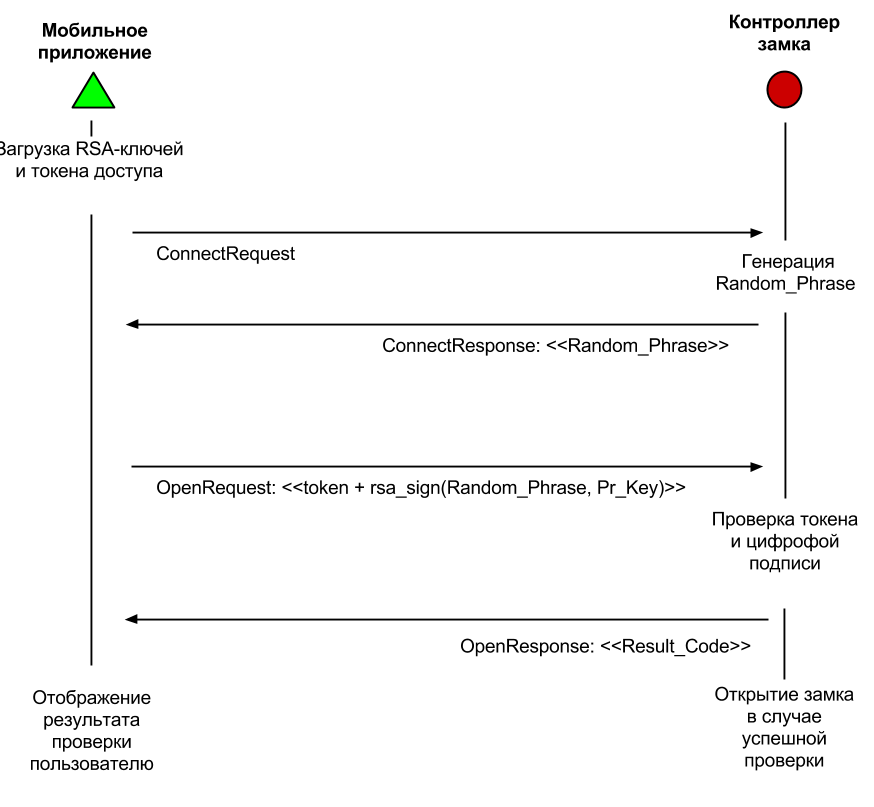
\includegraphics[scale=0.4]{mblock_open}\\ % Указывается размер рисунка (каким Вы его хотите видеть)% и имя вставляемого файла
	\caption{Открытие замка}% Подпись рисунка должна быть обязательно
	\label{mblock_open}% Метка для ссылки на рисунок.
\end{figure}

В ConnectResponse приложение контроллера замка генерирует случайную фраза. OpenRequest содержит token и цифровую подпись сгенерированной случайной фразы. Получив OpenRequest приложение контроллера замка производит дешифрование токена, и проверяет целостность контрольной фразы. В случае корректности контрольной фразы, приложение контроллера замка может быть уверено в валидности остальных данных. Приложение контроллера замка имеет возможность сравнить текущее время с Timestamp\_UTC, а также проверить верности цифровой подписи на основе. В случае если текущее время не превосходит Timestamp\_UTC и цифровая подпись верна, приложение контроллера замка подает на замок управляющую команду которая открывает замок. В случае ошибки, код ошибки возвращается в OpenResponse и мобильное приложение отображает пользователю информацию об ошибке и возможные пути к ее устранению.

\section{Вопросы безопасности} \label{subsect2_5}
В 2014 году приложениеланируется детальная экспертиза безопасности системы совместно с Лабораторией Касперского.
\clearpage